The approach taken by the authors for both the baseline and the industry-level study may be considered naive and outdated: as previously treated units are included in the subsequent control groups, the resulting estimate for the $\alpha_1$`s and $\beta_1$`s is a weighted average of the treatment effects for each group, with weights that may even be negative, and thus potentially biased.
To address this issue, I adopt a modern diff-in-diff technique proposed by~\textcite{callaway}, implemented in Stata in the \texttt{csdid} package.
It offers two primary advantages:
\begin{enumerate}
\item Enhanced Control Group Selection: It provides flexibility in choosing control groups.
Specifically, it allows to utilize \textit{not-yet treated units} as controls in addition to \textit{never-treated} units (as this dataset lacks never treated groups).
\item Covariate Incorporation: it accommodates the inclusion of covariates, thereby ensuring that the parallel conditions assumption holds conditionally on these covariates, and implicitly handling the fixed effects.
\end{enumerate}
In particular, I focus on evaluating the average treatment effect (ATT) by treatment group, reported in~\ref{tab:group}.
Moreover, I reproduce, in figure~\ref{fig:dynamic_att} the dynamics in the $(-5,10)$ year window around the enforcement year.

\subsection{Treatment Effect by Group}\label{subsec:staggered-treatment-estimate}
Table~\ref{tab:group} and its graphical representation in figure~\ref{fig:group_att} reproduce the average treatment effect for different groups, using the industry-level dataset.
A similar analysis has been performed on the country level dataset, and in both cases, the treatment effect are found to be not statistically relevant.

\begin{figure}[h!]
    \centering

    \begin{subfigure}[b]{0.40\textwidth}
        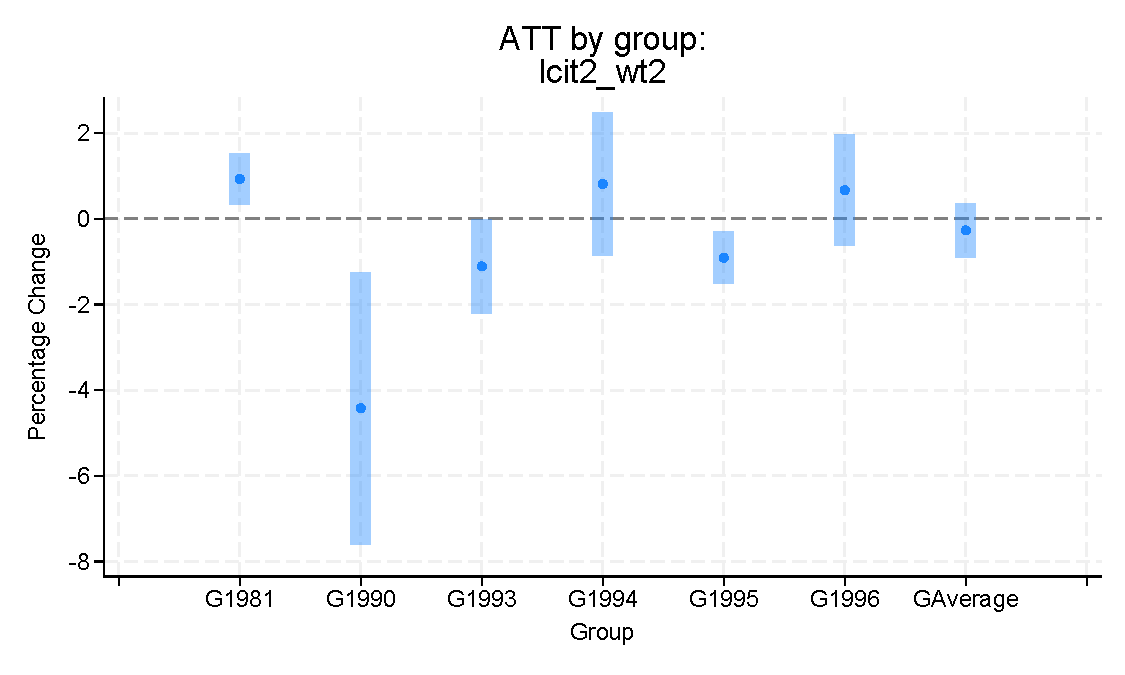
\includegraphics[width=\linewidth]{images/group_lcit2_wt2}
        \caption{Citation Weight}
    \end{subfigure}
    \hfill
    \begin{subfigure}[b]{0.40\textwidth}
        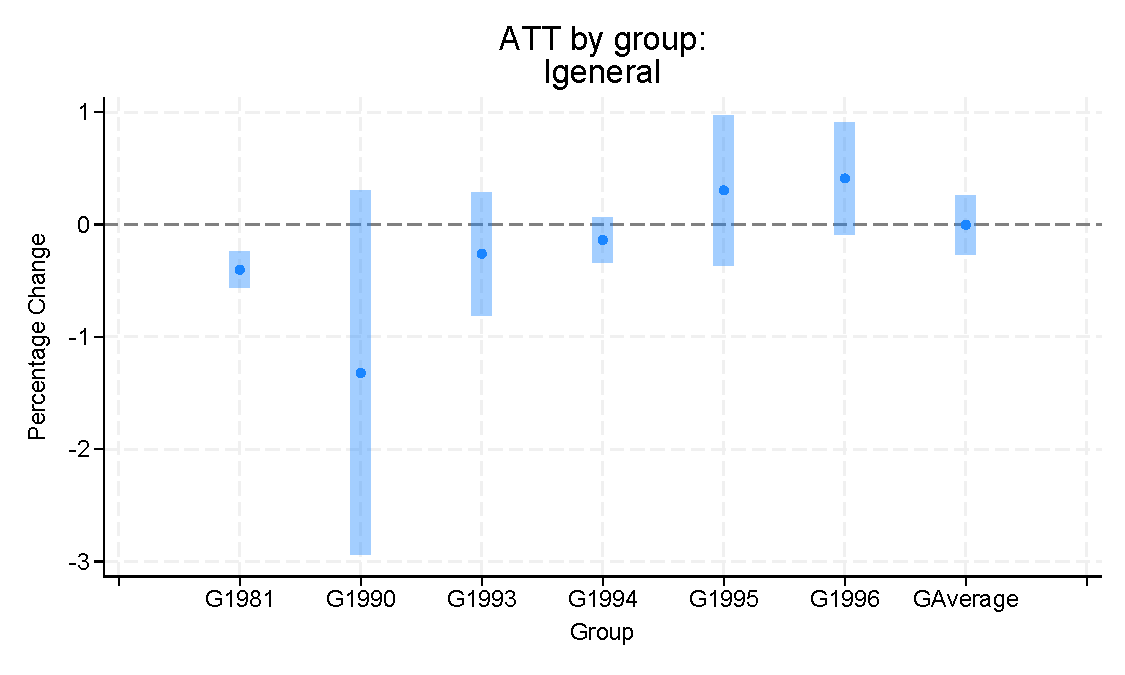
\includegraphics[width=\linewidth]{images/group_lgeneral}
        \caption{General Innovation}
    \end{subfigure}

    \vspace{0.4cm}

    \begin{subfigure}[b]{0.40\textwidth}
        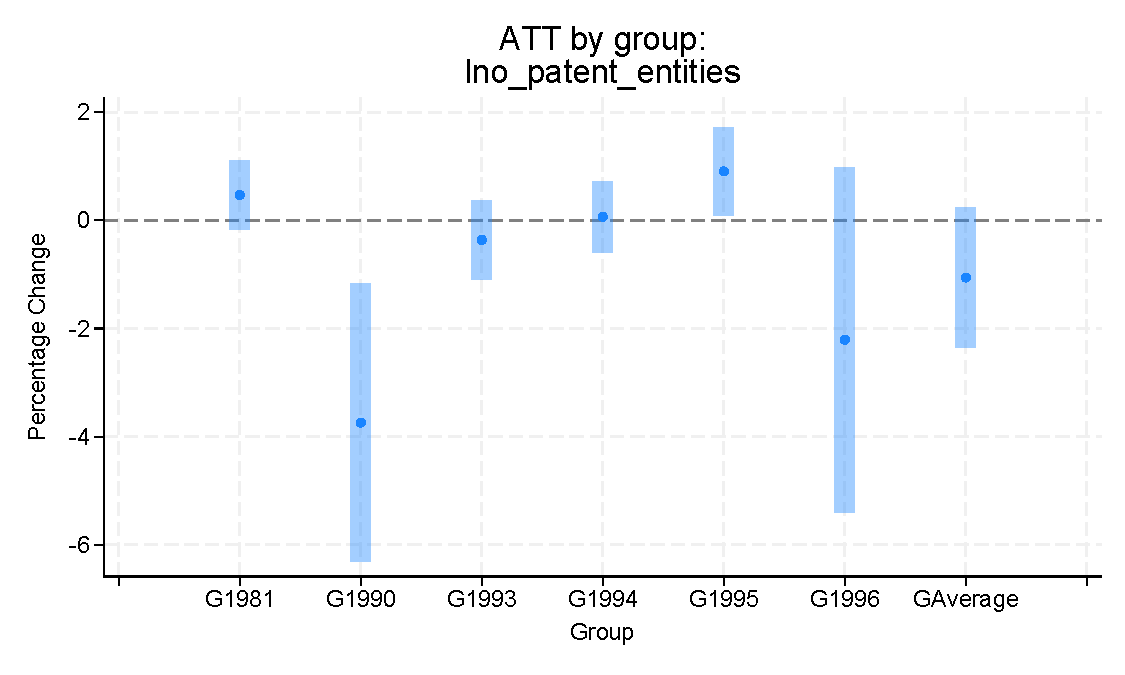
\includegraphics[width=\linewidth]{images/group_lno_patent_entities}
        \caption{Patent Entities}
    \end{subfigure}
    \hfill
    \begin{subfigure}[b]{0.45\textwidth}
        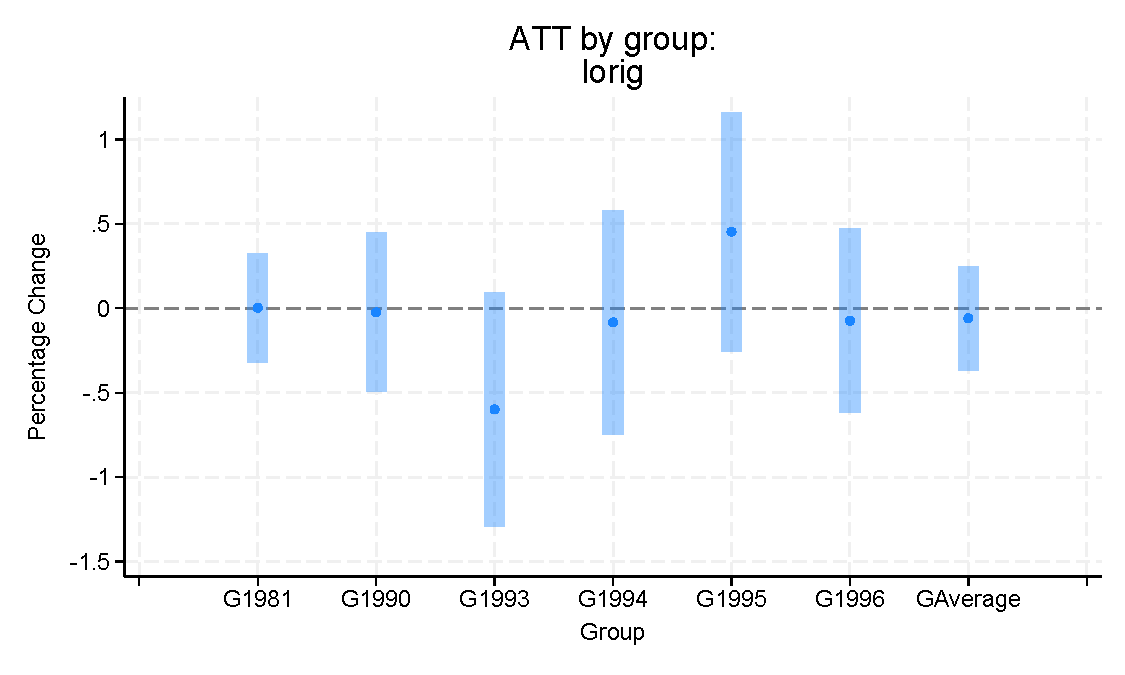
\includegraphics[width=\linewidth]{images/group_lorig}
        \caption{Originality}
    \end{subfigure}

    \vspace{0.4cm}

    \begin{subfigure}[b]{0.40\textwidth}
        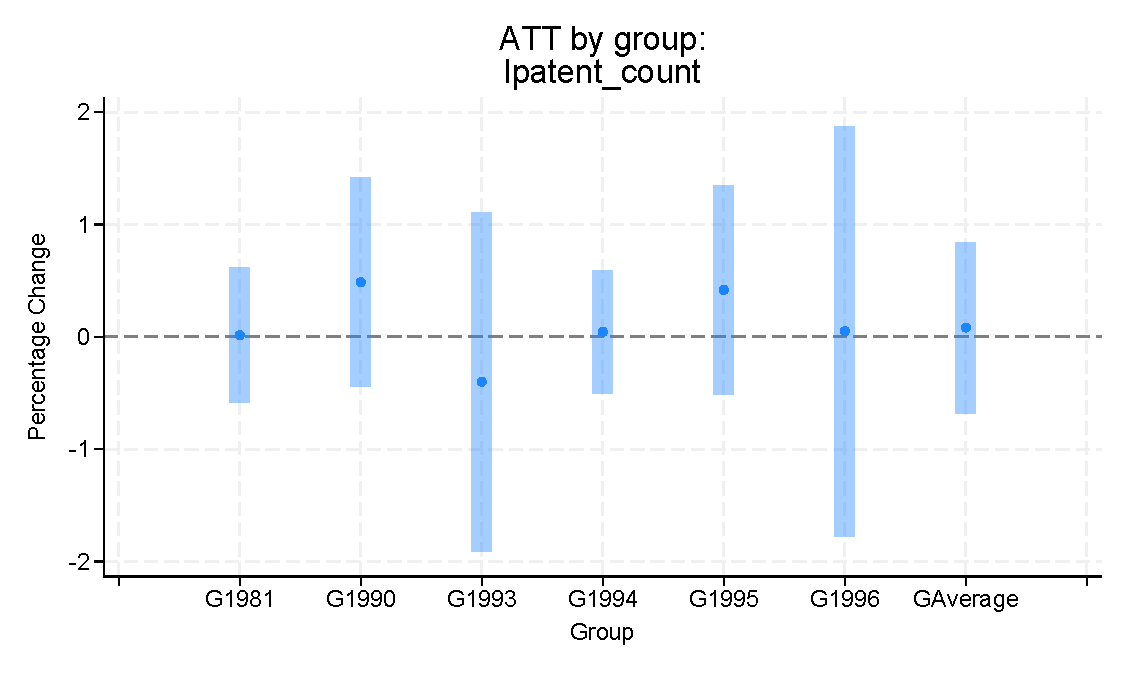
\includegraphics[width=\linewidth]{images/group_lpatent_count}
        \caption{Patent Count}
    \end{subfigure}
    \hfill
    \begin{subfigure}[b]{0.40\textwidth}
        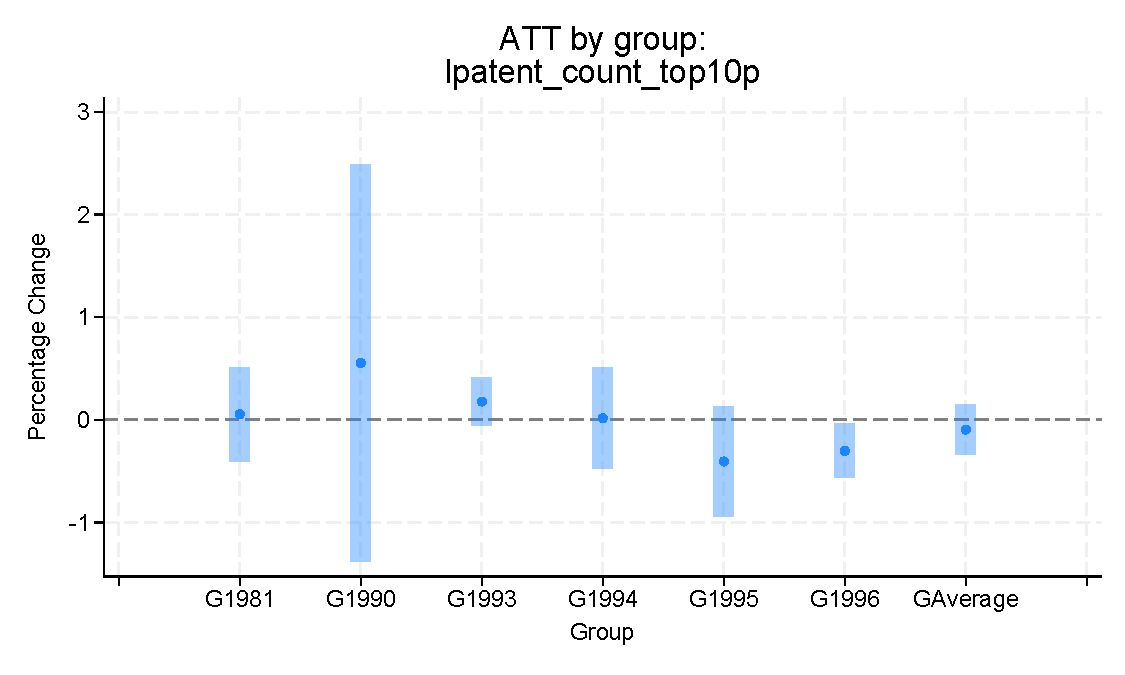
\includegraphics[width=\linewidth]{images/group_lpatent_count_top10p}
        \caption{Top 10\% Patents}
    \end{subfigure}

    \caption{ATT Estimates by Group Across Innovation Measures}
    \label{fig:group_att}
\end{figure}

\begin{landscape}
    \begin{table}[h!]
\centering
\caption{ATT by Group}
\label{tab:group}
\begin{tabular}{l*{6}{c}}
\hline\hline
                    &\multicolumn{1}{c}{(1)}&\multicolumn{1}{c}{(2)}&\multicolumn{1}{c}{(3)}&\multicolumn{1}{c}{(4)}&\multicolumn{1}{c}{(5)}&\multicolumn{1}{c}{(6)}\\
                    &\multicolumn{1}{c}{Patent Count}&\multicolumn{1}{c}{Patent Entities}&\multicolumn{1}{c}{Citation Weight}&\multicolumn{1}{c}{Top 10\% Patents}&\multicolumn{1}{c}{General Innovation}&\multicolumn{1}{c}{Originality}\\
\hline
GAverage            &      0.0823         &      -1.059         &      -0.270         &     -0.0946         &    -0.00366         &     -0.0588         \\
                    &     (0.388)         &     (0.657)         &     (0.326)         &     (0.124)         &     (0.134)         &     (0.157)         \\
[1em]
G1981               &      0.0141         &       0.469         &       0.933\sym{***}&      0.0542         &      -0.403\sym{***}&     0.00337         \\
                    &     (0.307)         &     (0.324)         &     (0.308)         &     (0.235)         &    (0.0810)         &     (0.165)         \\
[1em]
G1990               &       0.486         &      -3.740\sym{***}&      -4.424\sym{***}&       0.555         &      -1.322         &     -0.0240         \\
                    &     (0.473)         &     (1.310)         &     (1.618)         &     (0.987)         &     (0.826)         &     (0.241)         \\
[1em]
G1993               &      -0.400         &      -0.363         &      -1.111\sym{**} &       0.179         &      -0.262         &      -0.599\sym{*}  \\
                    &     (0.770)         &     (0.376)         &     (0.562)         &     (0.117)         &     (0.279)         &     (0.355)         \\
[1em]
G1994               &      0.0439         &      0.0655         &       0.814         &      0.0152         &      -0.138         &     -0.0832         \\
                    &     (0.281)         &     (0.335)         &     (0.857)         &     (0.251)         &     (0.103)         &     (0.338)         \\
[1em]
G1995               &       0.417         &       0.904\sym{**} &      -0.908\sym{***}&      -0.405         &       0.302         &       0.454         \\
                    &     (0.476)         &     (0.417)         &     (0.311)         &     (0.272)         &     (0.340)         &     (0.362)         \\
[1em]
G1996               &      0.0498         &      -2.207         &       0.668         &      -0.302\sym{**} &       0.409         &     -0.0736         \\
                    &     (0.930)         &     (1.626)         &     (0.659)         &     (0.135)         &     (0.254)         &     (0.278)         \\
\hline
Observations        &                     &                     &                     &                     &                     &                     \\
\hline\hline
\multicolumn{7}{l}{\footnotesize Standard errors in parentheses}\\
\multicolumn{7}{l}{\footnotesize \sym{*} \(p<0.10\), \sym{**} \(p<0.05\), \sym{***} \(p<0.01\)}\\
\end{tabular}
\end{table}


\end{landscape}


\subsection{Dynamics}\label{subsec:dynamics}
As reported in the following figure~\ref{fig:dynamic_att} and table~\ref{tab:dynamic_att}, also in the event aggregation of the $ATT(g,t)$ functions the effects are mostly statistically insignificant.

\begin{figure}[h!]
    \centering
    \begin{subfigure}[b]{0.45\textwidth}
        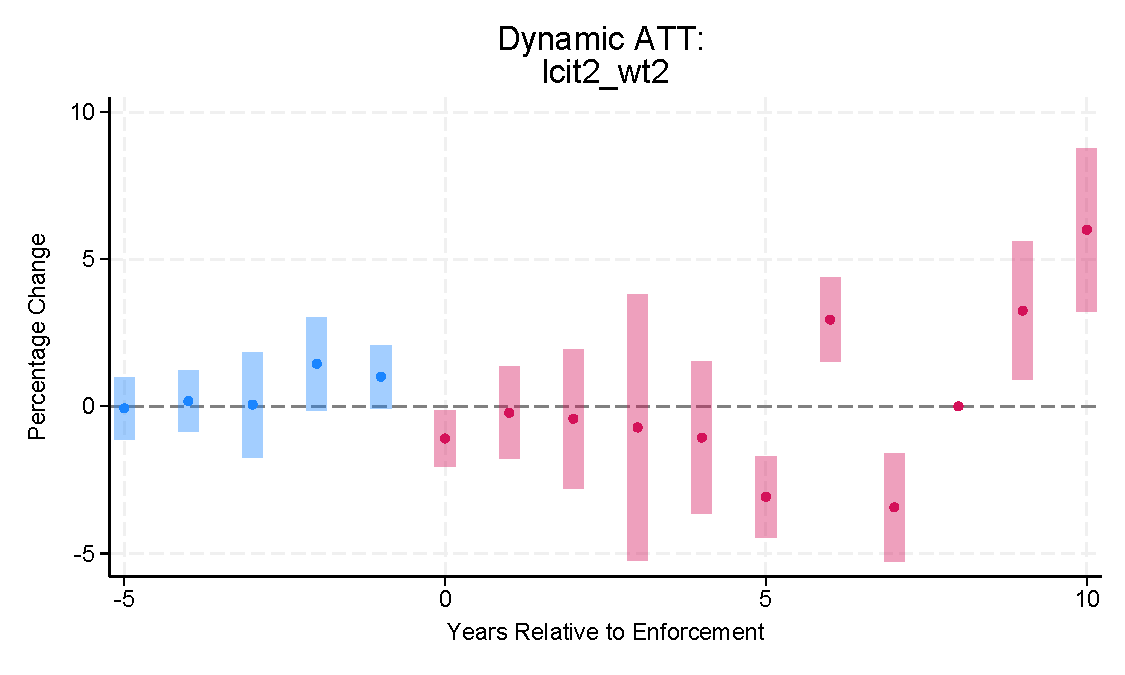
\includegraphics[width=\linewidth]{images/dynamic_att_lcit2_wt2}
        \caption{Citation Weight}
    \end{subfigure}
    \hfill
    \begin{subfigure}[b]{0.45\textwidth}
        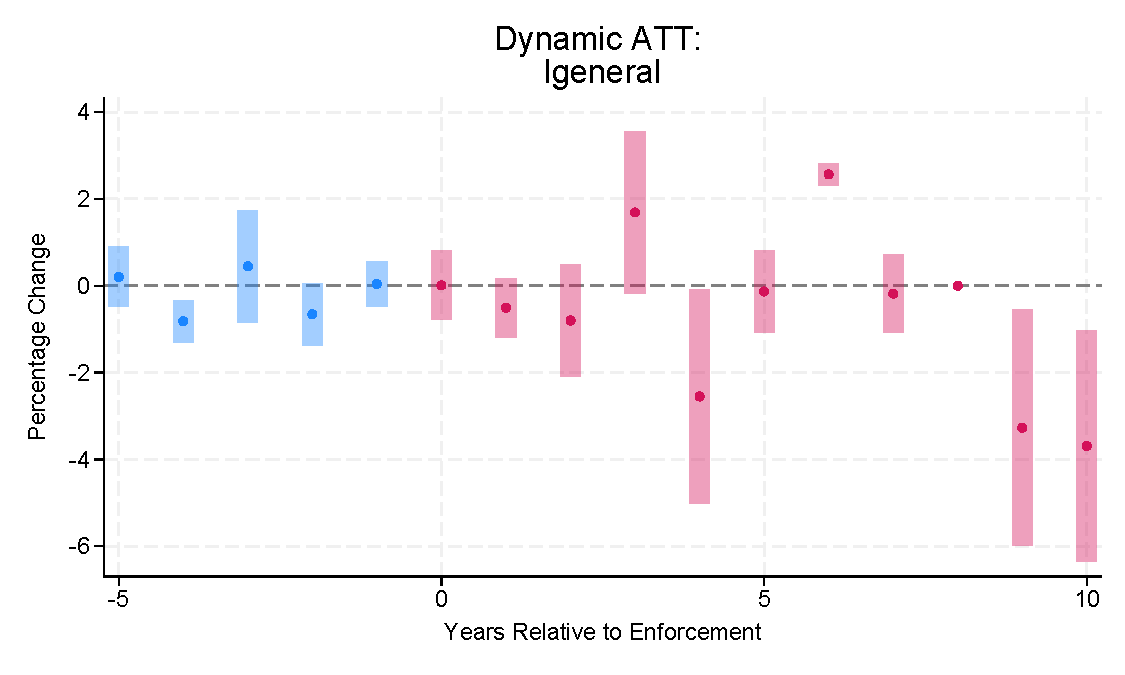
\includegraphics[width=\linewidth]{images/dynamic_att_lgeneral}
        \caption{General Innovation}
    \end{subfigure}

    \vspace{0.5cm}

    \begin{subfigure}[b]{0.45\textwidth}
        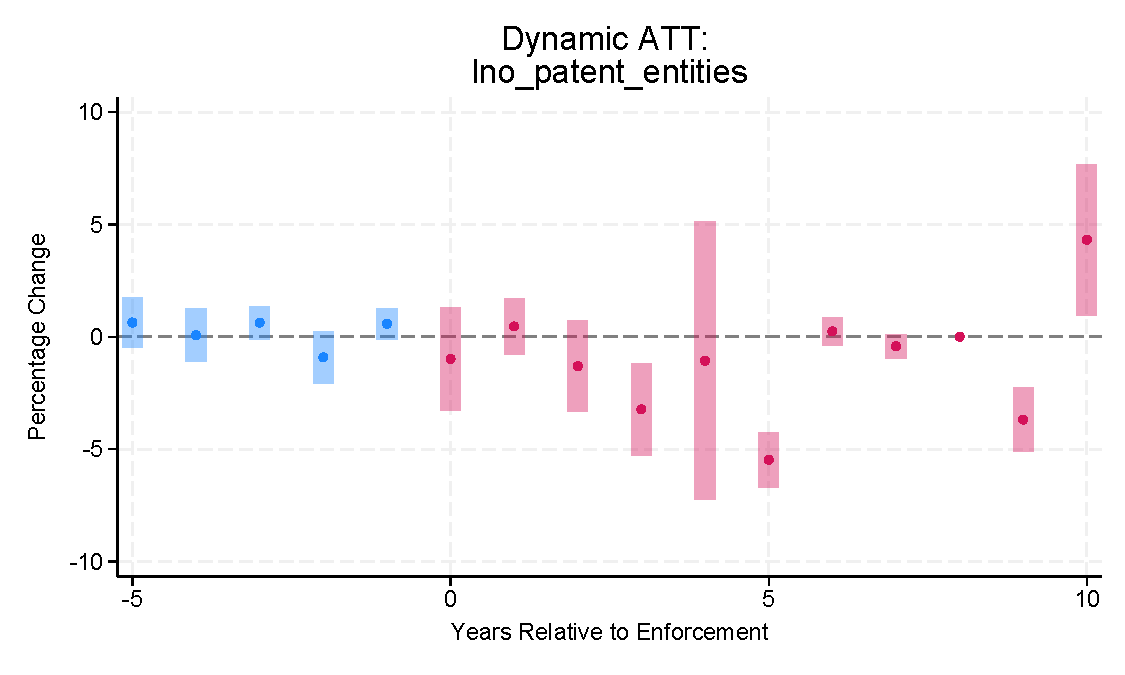
\includegraphics[width=\linewidth]{images/dynamic_att_lno_patent_entities}
        \caption{Patent Entities}
    \end{subfigure}
    \hfill
    \begin{subfigure}[b]{0.45\textwidth}
        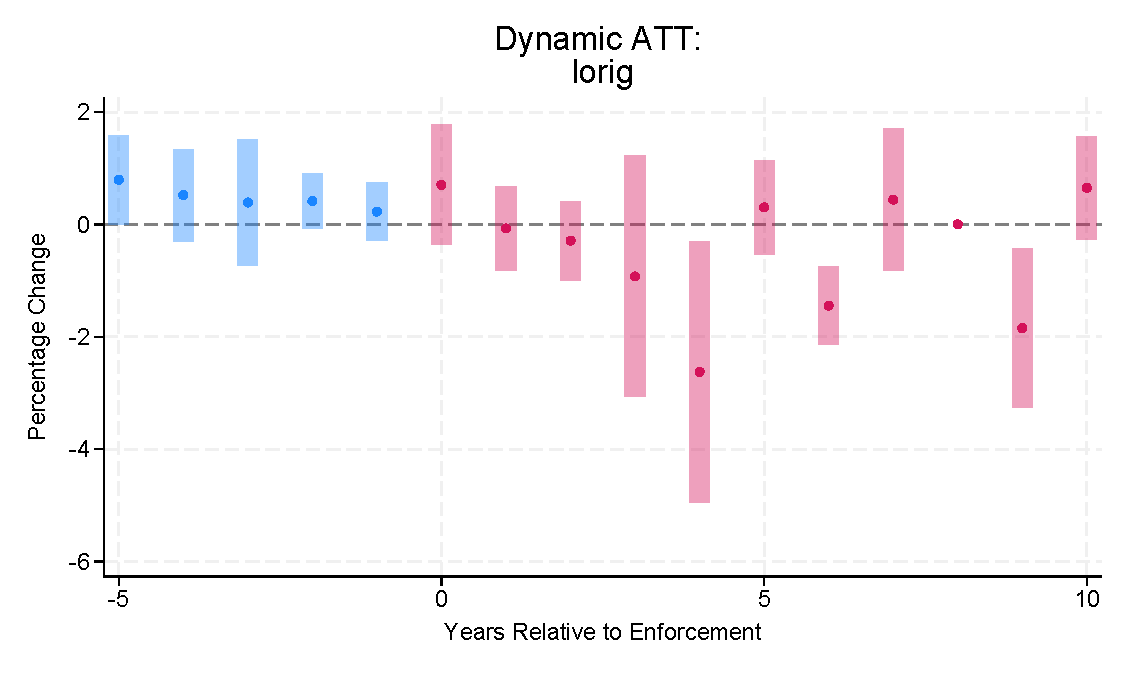
\includegraphics[width=\linewidth]{images/dynamic_att_lorig}
        \caption{Originality}
    \end{subfigure}

    \vspace{0.5cm}

    \begin{subfigure}[b]{0.45\textwidth}
        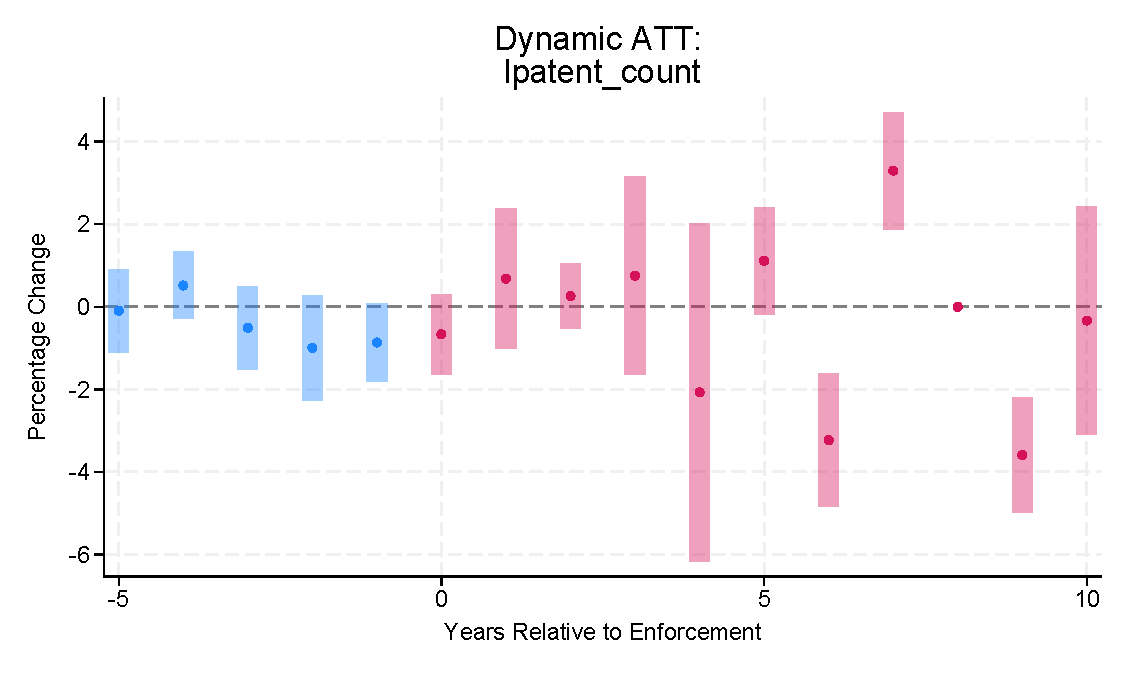
\includegraphics[width=\linewidth]{images/dynamic_att_lpatent_count}
        \caption{Patent Count}
    \end{subfigure}
    \hfill
    \begin{subfigure}[b]{0.45\textwidth}
        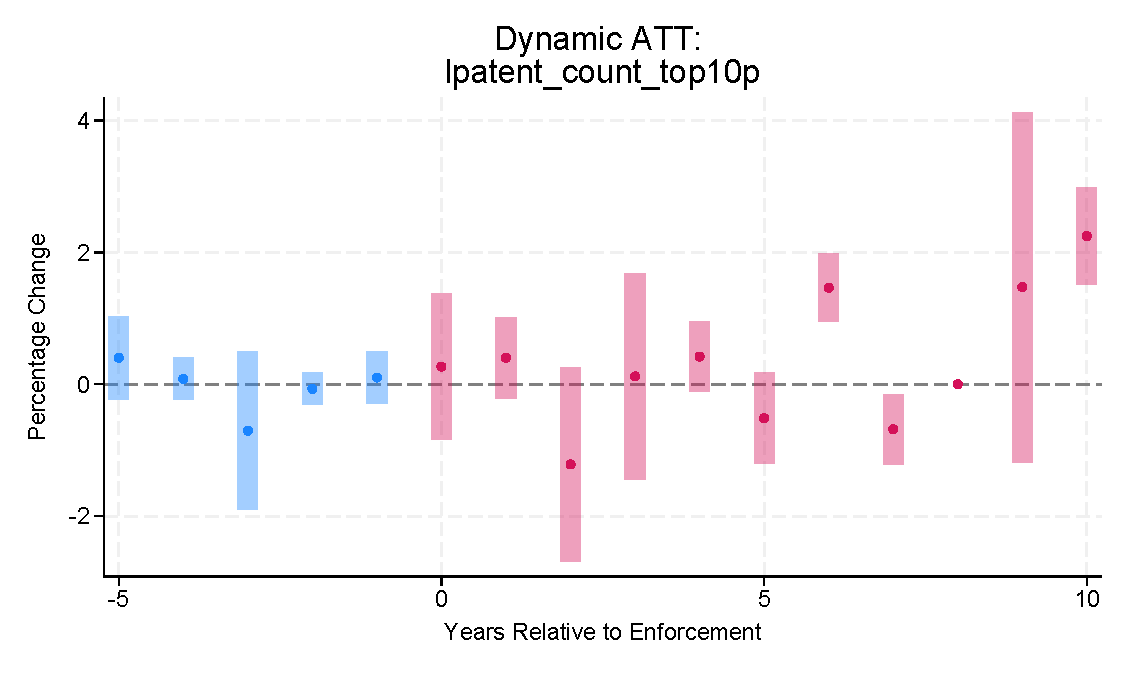
\includegraphics[width=\linewidth]{images/dynamic_att_lpatent_count_top10p}
        \caption{Top 10\% Patents}
    \end{subfigure}

    \caption{Dynamic ATT Estimates Across Innovation Measures}
    \label{fig:dynamic_att}
\end{figure}

\begin{landscape}
    \begin{longtable}{l*{6}{c}}
    \caption{Dynamic ATT by Event Time}
    \label{tab:dynamic_att} \\

\hline\hline
                    &\multicolumn{1}{c}{(1)}&\multicolumn{1}{c}{(2)}&\multicolumn{1}{c}{(3)}&\multicolumn{1}{c}{(4)}&\multicolumn{1}{c}{(5)}&\multicolumn{1}{c}{(6)}\\
                    &\multicolumn{1}{c}{Patent Count}&\multicolumn{1}{c}{Patent Entities}&\multicolumn{1}{c}{Citation Weight}&\multicolumn{1}{c}{Top 10\% Patents}&\multicolumn{1}{c}{General Innovation}&\multicolumn{1}{c}{Originality}\\
\hline
Pre\_avg            &      -0.389         &       0.199         &       0.523\sym{**} &     -0.0369         &      -0.157         &       0.470\sym{**} \\
                    &     (0.300)         &     (0.260)         &     (0.238)         &     (0.113)         &     (0.244)         &     (0.188)         \\
[1em]
Post\_avg           &           0         &           0         &           0         &           0         &           0         &           0         \\
                    &         (.)         &         (.)         &         (.)         &         (.)         &         (.)         &         (.)         \\
[1em]
Tm5                 &     -0.0947         &       0.635         &     -0.0709         &       0.402         &       0.203         &       0.795\sym{**} \\
                    &     (0.514)         &     (0.562)         &     (0.542)         &     (0.321)         &     (0.353)         &     (0.404)         \\
[1em]
Tm4                 &       0.517         &      0.0696         &       0.176         &      0.0820         &      -0.818\sym{***}&       0.521         \\
                    &     (0.414)         &     (0.598)         &     (0.526)         &     (0.163)         &     (0.246)         &     (0.417)         \\
[1em]
Tm3                 &      -0.508         &       0.631\sym{*}  &      0.0577         &      -0.703         &       0.447         &       0.391         \\
                    &     (0.516)         &     (0.374)         &     (0.910)         &     (0.610)         &     (0.659)         &     (0.574)         \\
[1em]
Tm2                 &      -0.995         &      -0.918         &       1.447\sym{*}  &     -0.0681         &      -0.657\sym{*}  &       0.416\sym{*}  \\
                    &     (0.646)         &     (0.598)         &     (0.809)         &     (0.122)         &     (0.365)         &     (0.248)         \\
[1em]
Tm1                 &      -0.864\sym{*}  &       0.576         &       1.007\sym{*}  &       0.102         &      0.0392         &       0.228         \\
                    &     (0.479)         &     (0.351)         &     (0.549)         &     (0.198)         &     (0.259)         &     (0.266)         \\
[1em]
Tp0                 &      -0.664         &      -0.982         &      -1.093\sym{**} &       0.267         &     0.00942         &       0.706         \\
                    &     (0.495)         &     (1.166)         &     (0.491)         &     (0.567)         &     (0.406)         &     (0.547)         \\
[1em]
Tp1                 &       0.683         &       0.459         &      -0.218         &       0.400         &      -0.507         &     -0.0711         \\
                    &     (0.869)         &     (0.639)         &     (0.802)         &     (0.312)         &     (0.349)         &     (0.381)         \\
[1em]
Tp2                 &       0.258         &      -1.308         &      -0.423         &      -1.215         &      -0.800         &      -0.290         \\
                    &     (0.401)         &     (1.034)         &     (1.206)         &     (0.751)         &     (0.663)         &     (0.359)         \\
[1em]
Tp3                 &       0.752         &      -3.226\sym{***}&      -0.720         &       0.120         &       1.688\sym{*}  &      -0.926         \\
                    &     (1.226)         &     (1.049)         &     (2.299)         &     (0.795)         &     (0.950)         &     (1.094)         \\
[1em]
Tp4                 &      -2.070         &      -1.072         &      -1.064         &       0.421         &      -2.550\sym{**} &      -2.626\sym{**} \\
                    &     (2.091)         &     (3.154)         &     (1.314)         &     (0.272)         &     (1.262)         &     (1.183)         \\
[1em]
Tp5                 &       1.115\sym{*}  &      -5.474\sym{***}&      -3.080\sym{***}&      -0.514         &      -0.133         &       0.302         \\
                    &     (0.663)         &     (0.620)         &     (0.709)         &     (0.350)         &     (0.476)         &     (0.423)         \\
[1em]
Tp6                 &      -3.230\sym{***}&       0.241         &       2.945\sym{***}&       1.464\sym{***}&       2.563\sym{***}&      -1.446\sym{***}\\
                    &     (0.821)         &     (0.311)         &     (0.728)         &     (0.263)         &     (0.130)         &     (0.356)         \\
[1em]
Tp7                 &       3.299\sym{***}&      -0.423         &      -3.436\sym{***}&      -0.682\sym{**} &      -0.181         &       0.441         \\
                    &     (0.724)         &     (0.272)         &     (0.938)         &     (0.269)         &     (0.463)         &     (0.647)         \\
[1em]
Tp8                 &           0         &           0         &           0         &           0         &           0         &           0         \\
                    &         (.)         &         (.)         &         (.)         &         (.)         &         (.)         &         (.)         \\
[1em]
Tp9                 &      -3.590\sym{***}&      -3.686\sym{***}&       3.249\sym{***}&       1.474         &      -3.271\sym{**} &      -1.847\sym{**} \\
                    &     (0.715)         &     (0.725)         &     (1.201)         &     (1.355)         &     (1.385)         &     (0.723)         \\
[1em]
Tp10                &      -0.333         &       4.320\sym{**} &       6.000\sym{***}&       2.248\sym{***}&      -3.692\sym{***}&       0.651         \\
                    &     (1.406)         &     (1.715)         &     (1.414)         &     (0.378)         &     (1.357)         &     (0.467)         \\
\hline
Observations        &                     &                     &                     &                     &                     &                     \\
\hline\hline
\multicolumn{7}{l}{\footnotesize Standard errors in parentheses}\\
\multicolumn{7}{l}{\footnotesize \sym{*} \(p<0.10\), \sym{**} \(p<0.05\), \sym{***} \(p<0.01\)}\\
\end{longtable}


\end{landscape}


\newpage